\documentclass[11pt]{amsart}
\usepackage{geometry}                % See geometry.pdf to learn the layout options. There are lots.
\geometry{letterpaper}                   % ... or a4paper or a5paper or ... 
%\geometry{landscape}                % Activate for for rotated page geometry
%\usepackage[parfill]{parskip}    % Activate to begin paragraphs with an empty line rather than an indent
\usepackage{graphicx}
\usepackage{amssymb}
\usepackage{epstopdf}
\DeclareGraphicsRule{.tif}{png}{.png}{`convert #1 `dirname #1`/`basename #1 .tif`.png}

\title{Confinement Induced Electron Capture}
\author{Charles H Martin and Robert Godes}
%\date{}                                           % Activate to display a given date or no date

\begin{document}
\maketitle
\section{Abstract}

We describe a Gedandkenexperiment in which a bare proton can capture an electron due soley to confinement. We first briefly review the aspects around bare electron proton capture.  We then provide a numerical solution of the Fermi VA-Theory for K-electron capture for an electron-proton pair confined in a classical box of size L. Interestingly, we find that the capture is most likely for L=0.004-0.009 Angstroms, well beyond the radius of the proton. 

\section{Background}


We briefly review orbital electron capture and some considerations, like environmental effects on the rate, that motivate this study.

\subsection{Orbital Electron Capture}
In 1935, Yukawa proposed that a proton, bound in an atomic nucleus,  could capture a low lying, bound atomic electron, transforming into a neutron, and releasing an electron neutrino [1,10]


$$p^{+}+\;e^{-}\rightarrow\;n^{0}\;+\;\bar{\nu}^{e}$$

K-electron capture usually occurs in unstable radioisotopes which lack the (nuclear binding) energy to decay by positron emission (standard Beta decay).   

We can not observe electron capture directly, so we rely upon conservation of energy and momentum. We observe orbital electron capture by it's relaxation processes.  It is usualy a K-shell electron, but maybe L or higher.  The nucleus may absorb some energy, becoming excited.  It then undergoes internal conversion.  During this, a higher lying, bound atomic electron is aborbed, and an X-ray, or Auger electron released [see Figure \ref{fig:ec1}].

\begin{figure}
   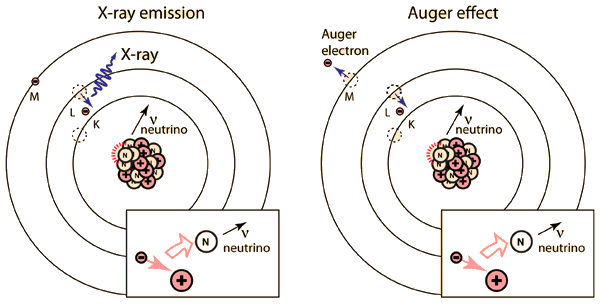
\includegraphics[scale=0.5]{img/ecrelax.png}
   \caption{oribital electon capture relaxation processes}
  \label{fig:ec1}
\end{figure}

Because electron capture occurs in (proton-rich) nuclei, and, subsequently, releases a X-Ray photon, the reaction is also sometimes written as

$$^{Z}X_{A}+\;e^{-}\rightarrow\;^{Z+1}X_{A-1}\;+\;h\nu_{X-ray}$$

(where Z is the number of protons, A the number of neutons, and $h\nu$ is an X-ray photon)

Indeed, orbital electron capture is evidenced by high intensity  x-rays and soft electrons.  In 1938, Luis W. Alvarez observed the x-ray signature of orbital electron capture in $^{48}V$ (in activated Titanium). Since then, electron capture has been observed in about 150 radioactive isotopes.


\subsubsection{Radiative Electron Capture}

In very rare cases, a gamma ray photon is emitted with the neutrino; this is called Radiative Electron Capture (REC) [10]. This can be thought of as a kind of Internal Bremsstrahlung radiation, caused by the electron accelerating toward the nucleus during capture. Recent, detailed rate calculatons have elucidated the details [11].

\subsubsection{Effect of Chemical Environment of Electron Capture rate} 
The lightest element that K-electron capture has been observed in is $^{7}Be$ [3]. In fact, there is so little energy that the competing positron emission process is not possible (described below), and the half-life for electron capture is $\tau_{EC}\sim 50\;days$.

Being so light, and having such a large rate, electron capture in $^{7}Be$ can be slighlty modified by both changing the chemical environment and/or the external pressure [4-6]. In particular, in 2004, Ohtsuki et al demonstrated a change of 0.83% by embedding Be in C-60 cages [6].
How could such changes occur ?

The electronic energy levels are in the eV range, so intense EM fields can alter the electronic structure and therefore slighly affect the rate. In contrast, the nuclear energy levels are in the keV to MeV region, and it is generally thought to be very difficult to impossible to effect.

Of particular practical interest is using very large electric fields for accelerating Beta decay for disposing of nuclear waste [?].

Generally speaking, rates of nuclear processes can be enhanced by providing additional avenues for energy release, thereby increasing the entropy of the total reaction. For example, in bound state $ \beta^{-} $ decay, the rate of decay is greatly enhanced in heavy, bare ions.  $^{187}Re$ decays with half life of $\tau_{\beta^{-}}\sim 42\times 10^{9}$ years, but fully ionized $^{187}Re^{+}_{75}$ undergoes bound state $\beta$ decay, with a half-life of only $\tau_{\beta^{-}}\sim\;32.9$ years. [7]

\subsection{The Weak Interaction and V-A theory}

Orbital electron capture is mediated by the Weak interaction. The simplest theory for the Weak Interaction is the Fermi V-A (Vector Axial) theory [8].
The V-A theory is a simple phenomenological approach, although it is now understood in terms of ElectroWeak Unification and can be derived from the Standard Model [9]. But we don't need all this machinary to do calculations.

One can use V-A theory to compute cross sections for scattering experiments and decay rates and electron capture for various atoms in chemical different environments.
To properly desrcibe any reaction, however, we need to understand what reactions we can apply the theory to, and the other reactions that might also occur.

\subsubsection{Electron Capture and other (weak) processes} 

The Weak interaction describes a variety of processes including:
\begin{itemize}
\item orbital (K) electron capture $\;\;\;\;\;\;\;\;\;\;p^{+}+e^{-} \rightarrow n^{0}+\nu_{e}\;\;,$

\item positon emission, or $\beta^{+}$ decay $\;\;\;\;\;p^{+}\rightarrow\;n^{0}+\;e^{+}\;+\;\nu_{e}\;\;,$

\item the related (electron) $\beta$ decay $\;\;;\;\;\;\;n^{0}\rightarrow p^{+}+\;e^{-}\;+\;\bar{\nu_{e}}$
\end{itemize}


A neutron-rich nucleus may undergo electron capture, positron emission, and/or $\beta$ decay, becoming more stable as a result.

\subsubsection{neutron decay}
Furthermore, there is the competing, reverse reaction, where a neutron interactions with a neutrino:
\begin{itemize}
\item reverse electon capture  $\;\;\;\;\;\;n^{0}+\nu_{e}\rightarrow p^{+}+e^{-}$.
\end{itemize}

By detailed balance, it has the same rate as orbital electron capture by a free proton, but is more favorable energetically.
This is similar to
\begin{itemize}
\item free neutron decay  $\;\;\;\;\;\;\;\;\;\;n^{0}\rightarrow p^{+}+e^{-}+\bar{\nu_{e}},$
\end{itemize}

Inside the nucleus, the neutron is stable. But, free neutron decay has mean lifetime of $\tau=881.5 1.5\;sec $, or about 15 minutes.
This is the for nuclei with high atomic number, which usually have more neutrons than protons.

In contrast, orbital electron capture by a free proton is unheardof outside of a stellar environments, so in order for orbital capture to occur by a free proton, some external energy is necessary, and the free neutron decay must be suppressed or kinetically unfavorable.
inverse beta decay

\subsubsection{inverse beta decay}

Note that K-electron capture is also sometimes called inverse $\beta$ decay, but we this to be the scatterinf of a proton and an electron anti-neutrino 

$$p^{+}+\bar{\nu_{e}} \rightarrow n^{0}+e^{+}\;\;,$$

and is characterized by emission of a positron. 

\subsubsection{positron emission}

In particular, any high energy relativisitc process, we have to worry about positron creation.  We noted above, however, that in $^{7}Be$, the competing positron decay reaction can not occue because there is not enough energy.    

Generally, this occurs at length scales below the Compton length of the electron, which, is smaller than we will need to consider.

\subsubsection{internal Bremsstrahlung}

Electron capture and Beta decay events may also emit Bremsstrahlung (or so-called *braking*) radiation, in the form of soft gamma rays. this is 1000X less likely, but does occur.  In electron capture, the electron emits this as it *accelerates* toward the nucleus, taking energy away from outbound neutrino.  The resulting gamma rays are called soft because they do not exhibit sharp spectral lines.  

\subsubsection{Rate calculations}

The rate of EC can be computed using the Fermi VA-Theory [8,10].  The most basic calculations require a only specifying the electronic wavefunctions(s), and integrating over the outbound neutrino momentum.  

Note that the V-A theory assumes an incoherent nuclear process, it is local, and that the interaction is phenomonological. It is treated as a simply a contact potential at the surface of the nucleus. This means one only needs compute the nuclear charge--the electron density on the surface of the nucleus.

More complicated calculations are used for larger nuclei, second order processes, etc. They only require modifications to treat either atomic electronic structure of reactant and product atoms, and/or specific considerations for nuclear internal conversion and other second order processes.

\end{document}  






